%!TEX root = ../my_thesis.tex
\chapter{Visualization of non-gridded data}

The most common way to render gridded data is using raster scan patterns. This technique steers the tip of the AFM on specific points of the grid. Past AFM research has been focused on improving those position controllers. Indeed, the AFM precision depends from the quality of the closed loop feedback on XY. These improvements, however, didn't solve fundamental problems with raster scanning. Most of the data is thrown away (border) and the actual position on the XY plane is inaccurate - and directly correlated with the efficiency of the position controller.

First, we discuss using sensor data instead of theoretical one and its implications in non-raster scanning. Then, we investigate how to render images from sparse data with Delaunay triangulation and inpainting. 

\section{Sensor data}
 
Current AFMs run in closed loop: position controllers on the XY axis are needed to steer the tip at the right position. 

Instead of using this method, we will work in open loop and register the data of the position sensors. One of the advantage of using sensor data is that we don't need accurate position controllers: it has no impact on our data. Instead of position the tip on an exact position, we're embracing its inaccuracy. The precision of our system is limited by the sensors and not the feedback on XY.

\section{Image rendering techniques}

Current AFMs give discrete data about the cantilever's position; therefore, we'll need to use image processing algorithms to generate images. The process of restoring is called inpainting. Indeed, it is mainly used to restore missing pieces in old paintings or photos. The principle behind inpainting is to fill a patch with its surroundings. An example of inpainting is removing an undesirable object from a picture. 

\subsection{Inpainting algorithms}

A common algorithm in image processing is to use heat equations to fill out patches of missing data on an image. The heat equation will distribute pixel value on its sides. The heat equation represents the distribution of heat in a region over time.

\begin{equation}\label{eqn:heateq}
\frac{\partial u}{\partial t} - \alpha \nabla^2 u = 0
\end{equation}


$\alpha$ is the thermal diffusivity - that is interpreted as a "thermal inertia modulus" - and $u$ is the temperature over space and time (i.e. $u(x,y,z,t)$). A high thermal diffusivity implies that the heat moves rapidly.

The algorithm has been implemented by /TRAVIS on MATLAB.

\cite{aubert2006mathematical} shows that heat equations are powerful to fill out these patches of missing data, but it smooths data on sharp edges(high frequency data). One of the effect is that edges are blurred out by the algorithm.


\subsection{OpenGL}

In this section, we see how to render images with OpenGL(Open Graphics Library). It is an API (Application Programming Interface) developed by Silicon Graphics to hide the complexities of interfacing with different 3D accelerators and mainly used for 3D modeling in video games and simulations. OpenGL leverages the fact that GPUs are optimized to render triangles.

\subsubsection{Triangulation with Delaunay}

The first problems we'll face when trying to plot our cloud of points is to know how to generate triangles. Indeed, OpenGL can only render triangles from a triplet of points. An unordered list of points will not be ordered by OpenGL. We'll need sophisticated algorithms like Delaunay triangulation to obtain those.
The principle behind the Delaunay triangulation is to generate triangles from triplets of point. 


The algorithm minimizes the angles of each triangle. The triangulation is successful if no vertex (i.e. 3-dimensional point) is in the interior of a triangle.

Triangle.c is a library developed in C by Jonathan Shewchuk \cite{shewchuk96b} to generate Delaunay triangulations. In our case, we'll only use the triangulation program on the first two dimensions of the 3d cloud of points. Indeed, we'll only render triangles on the 2D plane. We use the z-data to render the color of the image.

/IMAGE TRIANGLE OFFSET


\subsubsection{Immediate mode vs VBO}

We'll investigate two ways to render our surface with OpenGL: the immediate mode and vertex buffer objects.

The immediate mode is the simplest implementation of OpenGL. Indeed, we render  every frame. If we rotate the our 3D model, we'll have to regenerate the latter. The power of the immediate mode is its simple implementation (no initialization and extra code). Moreover, it is easier to debug. For a small number of vertices (< 10'000) the immediate mode is appropriate. \cite{opengl1} states that the immediate mode is more convenient and less overhead than other implementations (Vertex Buffer Objects)

The following code is an example of the immediate mode for a simple triangle. The display function is called when GLUT(OpenGL Utility Toolkit) determines that the windows needs to be redisplayed. Action like rotation, translation or resizing of the model will trigger the display event. Each time the display function will be called, the program will upload the vertices to the GPU.

This implementation is easy to understand and debug. Unfortunately, it is not the most efficient one. 

If we try to display a significant number of triangles (> 10'000 vertices), the CPU will be the bottle neck. The GPU doesn't start rendering data before glEnd. Thus, the CPU is spoon-feeding the GPU by transferring the data triangle by triangle. Moreover, the number of API calls is proportional to the number of triangles. I.e. if you have 10 triangles you will make (10*(2+3+3)) 80 API calls \cite{opengllegacy}. In conclusion, if you want to render less than 10'000 vertices, code a quick implementation and are not planning on making a lot of changes in your rendering, the immediate mode is the way to go.


One of the problem we have encountered with the immediate mode is the transfer from the system memory to the GPU.  We've seen there is a bottle neck in the transfer. With 10'000 points we can only have 3 frames per seconds. It means that our computer takes 300ms to upload our data to the GPU.

Instead of transferring the data from the memory to the GPU, the GPU could read the memory of the program. Buffer objects have been created to allow the GPU to have access to the memory. The process of reading the memory from the GPU is called Direct Memory Access (DMA). A buffer object is a contiguous untyped memory which the CPU and the GPU have access to.

We can't just upload our data into the memory without any structure. We need to map the data and make it readable for the GPU. We store our data in a vertex array object.

\begin{figure}[H]
  \centering
  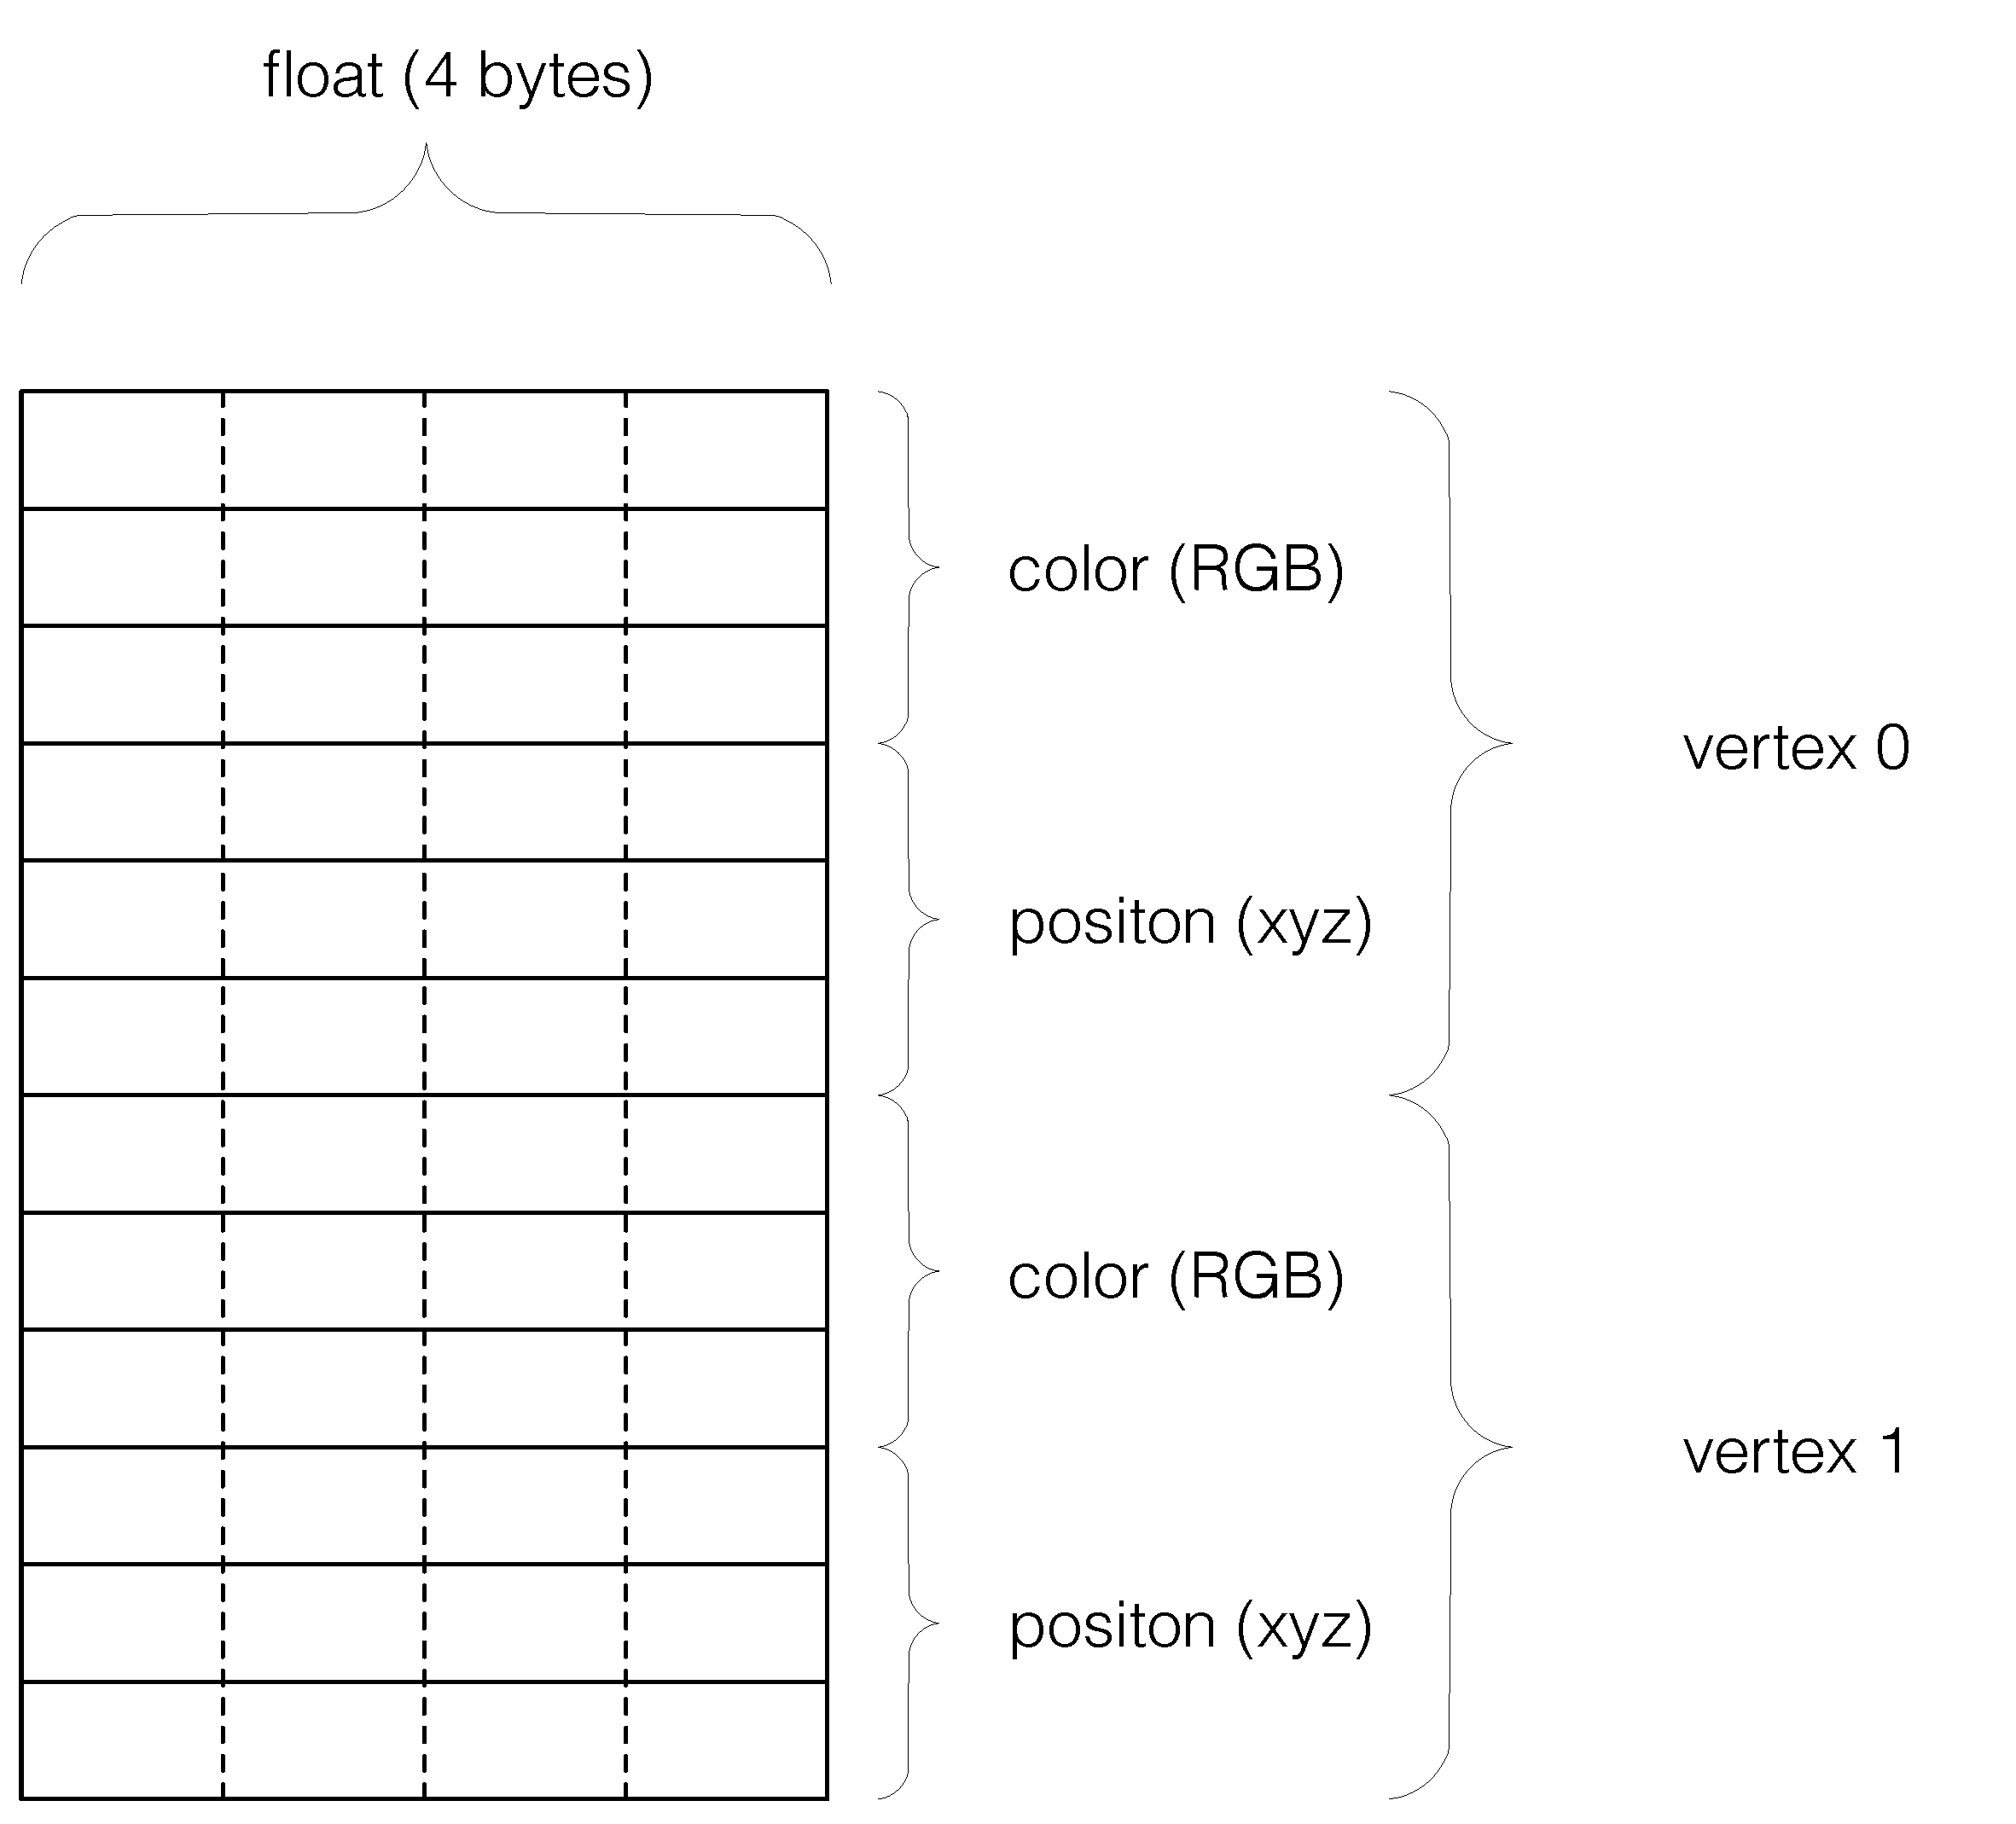
\includegraphics[scale=0.2]{images/memory.eps}
    \caption{Memory for the VAO}
  \label{memoryVAO}
\end{figure}


After having allocated and created this chunk of data, we need to map it to make it readable to the GPU. OpenGL has API calls for that application.

The advantage of this implementation is that you directly pull your data to a shared memory between the CPU and the GPU. Your CPU will spend less cycles making API calls thus improving the performances of the program. The power of the VBOs is that you just need to upload your data and your display function will just bind the VBO. Our performances have improved from 3FPS to 130FPS.

When we render 3D models from AFM scan we'll see that VBOs have smoothers animations.


\begin{table}[ht]
\caption{Rendering results[ms]} % title of Table
\centering % used for centering table
\begin{tabular}{c c c} % centered columns (4 columns)
\hline\hline %inserts double horizontal lines
 Nb of points & Delaunay & VBO \\ [0.5ex] % inserts table 
%heading
\hline % inserts single horizontal line

1000 & 2.9 & 23.9 \\
10000 & 8.1	&	27 	\\
100000 & 66.9 & 181 \\
1000000 & 640.7	& 267 \\[1ex]


\hline %inserts single line
\end{tabular}
\label{table:nonlin} % is used to refer this table in the text
\end{table}


